% !TEX TS-program = pdflatex
% !TEX encoding = UTF-8 Unicode

% This is a simple template for a LaTeX document using the "article" class.
% See "book", "report", "letter" for other types of document.

\documentclass[11pt]{scrartcl} % use larger type; default would be 10pt

\usepackage[utf8]{inputenc} % set input encoding (not needed with XeLaTeX)
%%% Examples of Article customizations
% These packages are optional, depending whether you want the features they provide.
% See the LaTeX Companion or other references for full information.

%%% PAGE DIMENSIONS
\usepackage{geometry} % to change the page dimensions
\geometry{a4paper} % or letterpaper (US) or a5paper or....
% \geometry{landscape} % set up the page for landscape
%   read geometry.pdf for detailed page layout information

\usepackage{graphicx} % support the \includegraphics command and options

% \usepackage[parfill]{parskip} % Activate to begin paragraphs with an empty line rather than an indent

%%% PACKAGES
\usepackage{booktabs} % for much better looking tables
\usepackage{array} % for better arrays (eg matrices) in maths
\usepackage{paralist} % very flexible & customisable lists (eg. enumerate/itemize, etc.)
\usepackage{verbatim} % adds environment for commenting out blocks of text & for better verbatim
\usepackage{subfig} % make it possible to include more than one captioned figure/table in a single float
\usepackage{amsfonts}
\usepackage{amsmath}% http://ctan.org/pkg/amsmath
\usepackage{amssymb}
\usepackage{amsthm}
\usepackage{listings}
\usepackage{hyperref}
\usepackage{float}
\usepackage{tcolorbox}
\usepackage{color}

\usepackage{pbox}
% These packages are all incorporated in the memoir class to one degree or another...

%%% HEADERS & FOOTERS
\usepackage{fancyhdr} % This should be set AFTER setting up the page geometry
\pagestyle{fancy} % options: empty , plain , fancy
\renewcommand{\headrulewidth}{0pt} % customise the layout...
\lhead{}\chead{}\rhead{}
\lfoot{}\cfoot{\thepage}\rfoot{}

%%% SECTION TITLE APPEARANCE
\usepackage{sectsty}
\allsectionsfont{\sffamily\mdseries\upshape} % (See the fntguide.pdf for font help)
% (This matches ConTeXt defaults)

%%% ToC (table of contents) APPEARANCE
\usepackage[nottoc,notlof,notlot]{tocbibind} % Put the bibliography in the ToC
\usepackage[titles,subfigure]{tocloft} % Alter the style of the Table of Contents
\renewcommand{\cftsecfont}{\rmfamily\mdseries\upshape}
\renewcommand{\cftsecpagefont}{\rmfamily\mdseries\upshape} % No bold!
\DeclareMathOperator*{\argmin}{arg\,min}

\lstset{frame=tb,
  aboveskip=3mm,
  belowskip=3mm,
  showstringspaces=false,
  columns=flexible}

\theoremstyle{plain}
\newtheorem{theorem}{Theorem}[section]
\newtheorem{lemma}[theorem]{Lemma}
%%% END Article customizations
\linespread{1.3}
%%% The "real" document content comes below...
\begin{document}

\begin{titlepage}
	\centering
	{\scshape\LARGE University of Washington\par}
	\vspace{1.5cm}
	{\huge\bfseries Practical Applications of Robust Principal Component Analysis\par}
	\vspace{2cm}
	{\Large\itshape  An Analysis by Jonathan Donovan \& Si Latt\par}

	\vfill

% Bottom of the page
	{\itshape Code can be found at \href{https://github.com/Cynocracy/principal-component-analysis}{our github} \par}
	{\large \today\par}
\end{titlepage}


\section{Abstract}
In this paper we analyze the performance of Principal Component Analysis (PCA) and Robust Principal Component Analysis (RPCA) on datasets that are artificially made noisy. In particular, we use a method\cite{pcp} which attempts to decompose the corrupted matrix into a low rank and a sparse component. The low rank component can then be used to recover the principal components for the data being analyzed. We attempted this on facial data (to recover eigenfaces) and on video data (as background recovery) and examined the performance of RPCA for each of these applications. The full results of this analysis and the code used can be found on \href{https://github.com/Cynocracy/principal-component-analysis}{our github project}.

\section{Introduction}

\subsection{Principal Component Analysis}

\[ PCA(M, k) =\argmin_{M'}(||M-M'||_F ) \mid rank(M') \le k \]

Principle Component Analysis\cite{pca} (or PCA) is the attempt to approximate a matrix $M$ with a nearby (in the Frobenius norm) low rank matrix $M'$. As a reminder, the rank of a matrix $M$ is the number of independent vectors that are needed to recreate the columns of the matrix, and the Frobenius norm of a matrix is a generalization of the euclidean norm for vectors, where $||A||_F = \sqrt{\sum_{a_{i,j} \in A}|a_{i,j}|^2}$.

When the columns of the matrix we are performing PCA on represent a series of measurements (usually with the average subtracted out), with PCA we are essentially trying to decompose the measurements into linearly independent 'hidden variables'. If we have reason to believe that our measurements are the result of a smaller subset of independent variables, PCA gives us the tools needed to find the best set of these variables.

PCA would not be useful if it were costly to compute, but thankfully, the problem formulation listed above is intimately related to a common operation in the analysis of matrices, that is: the Singular Value Decomposition. The Singular Value Decomposition (SVD) problem is a problem with the goal of decomposing a matrix into $M = U\Sigma V^*$, where $U$ and $V$ are unitary matrices ($UU^* = I$ and $V^*V = I$) and $\Sigma$ is a real diagonal matrix with the entries sorted. While the factorization may not be unique, the diagonal matrix is, and it can be shown that the best $k$-rank approximation of a matrix $M$ can be found as $M' = U \Sigma' V^*$ where $\Sigma'$ is the diagonal matrix $\Sigma$ with all entries $\sigma_{i,i} = 0$ for $i > k$. It suffices here to say that the SVD problem is well studied, and that solutions can be found quite quickly in $O(mn^2)$ time for an $m{\times}n$ matrix. Probabilstic methods exist which can perform even faster when $k << m, n$.

\subsection{Robust Principal Component Analysis}

Robust Principal Component Analysis (RPCA) \cite{pcp} is an extension of PCA to the domain of corrupted data. PCA can quite easily recognize data where redundancy in the information of the data points exists, but it does not properly account for the fact that the collection of data itself may be lossy. One circumstance in which PCA fails is where significant outliers exist in the data, where the inclusion of a single dramatic outlier may have a dramatic impact on the estimated principal components. In a world where massive amounts of data exist to be sample, but where the quality of the data may vary significantly, a variation on PCA which incorporates robustness to these problems adds significant utility when analyzing data with the intent of discovering low rank approximations.

In the paper "Robust principal component analysis?"\cite{pcp} such a method is outlined, called Principal Component Pursuit (PCP). PCP breaks down the finding of the solution into decomposing a given matrix $M$ into two components $L$ and $S$ via the equation:

\[
L, S = \argmin_{L, S}(||L||_* + \lambda ||S||_1) \mid L + S = M
\]

where $||A||_*$ is the nuclear norm, defined as the sum of the singular values of M, or $\sum_{\sigma \in SVD(M)} \sigma$, and $||A||_1$ is the sum of the absolute values of the entries of $A$, or $\sum_{a_{i,j} \in A} |a_{i,j}|$. Amazingly, as part of the analysis the authors determine that there is a choice of parameter $\lambda = \frac{1}{\sqrt{n}}$ that succeeds with fairly high probability. To be specific this algorithm succeeds perfectly capture the original matrices $L$ and $S$ with $P \ge 1 - \frac{c}{n^10}$ provided the conditions that (for an $n{\times}n$ matrix)

\[
rank(L) \le \frac{p_r n}{\mu (log n)^2} \text{ and } m \le p_s n^2
\]

Here $p_r$ and $p_s$ are positive constants, $\mu$ is a measure of incoherence\cite{incoherence} (with small $\mu$ it is required that the significant values are not sparse), and $m$ is the support set of the matrix $S_0$ (or equivalently, the number of nonzero entries in $S_0$). Interestingly, this shows that the number of corrupted entries can scale linearly with the size of the matrix, and that with a fixed $\mu$, the rank of the low rank component $L_0$ can grow as $\frac{n}{log(n)^2}$. Another interesting point to note is that while we have constraints on the number of corrupted entries (the support set of $S_0$) we have no such constraints on how the data is corrupted (that is, it could be corrupted with arbitrarily large absolute value errors). When in fact our goal in many circumstances is to recover a fixed low rank approximation from a large amount of (probabilistically corrupted) data, these constraints work perfectly!

However one difficulty with this algorithm is that, while provably able to separate low rank from sparse data, it has not performed as succesfully on real world data, frequently taking a large number of iterations to complete. An alternative algorithm is described in \cite{iaml}, the Inexact Augment Lagrange Multiplier method. This algorithm has no proof of correctness, but uses a relaxed form of the constraints above. by solving the lagrangian problem:

\[
F(L, S, Y, \mu) = ||L||_* + \lambda ||S||_1 + <Y, M - L - S> + \frac{\mu}{2}||M-L-S||_F^2
\]

In addition, it uses an iterative approach towards updating the $S$ and $Y$ matrices that limits the number of SVD operations necessary for the algorithm to succeed. While this algorithm has not been proven correct, the fact that it is much faster in practice, and has been shown to converge in many practical demonstrations, we will use this algorithm when analyzing the performance of RPCA on our datasets. One important feature to note, is that it is recommended that $\mu_0$ be set to $\frac{1.25}{||M||_2}$.

During the analysis section of this paper, we primarily used code obtained from \cite{usedcode}, which is a translation of the MATLAB implementation of RPCA into numpy created by Kyle Kastner.

\section{Potential Uses for RPCA}

\subsection{Facial Identification}
One area we would like to investigate more thoroughly here, is the impact that RPCA has on the use of eigenfaces. Eigenfaces are the result of an attempt to use the low dimensional structure of facial images to create a small number of 'basis faces' that can be used to segment pictures of individuals, allowing identification of individuals based on a small number of projections. One property of image data in general that makes it quite amenable to PCA analysis is that the dimensions are naturally bounded (by 0 and 255 in most formats), meaning that no renormalization of particular dimensions needs to take place in order for PCA to find reasonable latent variables.

There is another property of facial data that makes it an attractive target for PCA: it has been shown that an idealized Lambertian convex surface (that is, a convex surface that has an ideal matte appearance) when displayed with arbitrary illuminations, lies on a 9 dimensional subspace\cite{lambertian}. While faces are neither perfectly Lambertian nor perfectly convex, the fact that they may be approximated as such lends credence to the idea that analyzing a particular face (or group of faces) may involve looking for low dimensional data underlying the apparently complex representation of the images themselves (which can be on the order of thousands or even millions of pixels).

RPCA has been shown to be capable of correctly identifying specularities in facial image data of a particular individual in the past\cite{rpca}. As part of our research, we will attempt to determine whether RPCA lends itself to analyzing large data sets of facial data with many different lighting circumstances. If the promises of the approach are to be believed, it should be capable of recognizing the irregularities caused by these circumstances and correcting for them, allowing for more accurate eigenfaces to be collected once the sparse error component is eliminated.

\section{Video Segmentation}

One area where RPCA is commonly used is in video surveillance. In surveillance videos, each frame can be considered as having two major components - the static background and the moving, sparse foreground objects. Recall that RPCA decomposes the original matrix M into two parts, the low rank part L and the sparse part, S. Therefore, for video surveillance, background can be modeled as the low rank component L and the foreground objects can be modeled as the sparse component, S.

Turns out, naïve PCA can also be used for separating video background and foreground objects since background remains largely the same across frames and PCA can provide a robust probability distribution of the background. However, PCA is known to be susceptible to noise and we think it is interesting to explore how this naïve PCA modeling of background and foreground compare against RPCA and in the process, gain more insights into how RPCA works and how it complements PCA.

\section{Metrics}
The remainder of our paper will be spent analyzing the performance of RPCA relative to PCA on various data sets. In order to do so we would like to define a few metrics that would be useful when discussing the accuracy of RPCA in reproducing the original low rank matrix.

\subsection{Frobenius error}
One useful metric, and the one used by the original paper, was the metric $\frac{||L_0 - L||_F}{||L_0||_F}$, where $L_0$ is the true low rank matrix, and $L$ is the approximation that results from applying RPCA. This is a reasonable metric of the error of the approximation, as it is the sum of square errors of the approximation over the sum of squares of the values of the original matrix, giving a natural sense of 'how far' the resulting approximation lies from the true low rank matrix.

One difficulty with using this form of error, while it is the most common type used in papers discussing the RPCA problem, is that when using real world data, the true low rank matrix is not known, only the original matrix $M$. Replacing $L_0$ with $M$ above results in the metric becomign $\frac{||E||_F}{||M||_F}$, or to restate another way, measures that the sum of the squares of the error matrix derived relative to the original matrix. This can be used to determine whether the RPCA algorithm has successfully found a relatively small error in it's decomposition, but does not give us much indication into how well it performed (that is, whether the low rank matrix obtained is truly indicative of the data underlying the metrics).

\subsection{Clustering Metric}

In the particular case of eigenfaces, one stated goal of the creation of the eigenfaces involved is to allow for easy recognition of particular people. As such, we could evaluate how well our eigenfaces perform based on how well they correctly cause images of the same person to be clustered close together. Let us call $v_1 .. v_k$ to be the projection of a particular image onto the first to the kth eigenface generated either Robust or standard PCA, which is a natural dimensionality reduction often used to analyze PCA performance.

We can evaluate how well our data is clustered within the projection by using the silhouette width\cite{silhouette} for the clusters in the new projected space. Assuming we have mapped each metric into the basis provided by the k eigenfaces (let us call these mapped vectors objects $o_1 .. o_m$), we can define our clusters $C_1 .. C_n$ to be the natural clusters formed when clustering all images of the same individual.

We can define $a(o_i)$ to be the average distance of the object $o_i$ within it's cluster, $b(o_i)$ to the minimum over all other clusters of average distance to that cluster, and the silhouette distance for that object to be the difference of those measures over the maximum.

\[
a(o_i) = \frac{1}{|C_{o_i}| - 1} \sum_{o_j \in C_{o_i}, o_j \ne o_i} d(o_i, o_j)
\]

\[
b(o_i) = \min_{C_B \ne C_{o_i}} \frac{1}{|C_B|} \sum_{o_j \in C_B} d(o_i, o_j)
\]

\[
sil(o_i) = \frac{b(o_i) - a(o_i)}{\max{a(o_i), b(o_i)}}
\]

Then, the silhouette width of the a cluster is naturally defined as the average silhouette width of the objects within it, and the width of the entire clustering to be the average over its clusters.
 
\[
sil(C_i) = \frac{1}{|C_i|}\sum_{o_j \in C_i} sil(o_j)
\]

\[
sil(C) = \frac{1}{n}\sum_{i = 1}^{n} sil(C_i)
\]

In general, the silhouette width is a number from -1 to 1 indicating how close the clusters are. If the number is 1, the in-cluster distances are infinitely closer than the between cluster distances. A number below 0 tends to indicate that there are more natural clusters, as the average object is closer to a different cluster than the one it was placed in. In addition, the silhouette score can be used with any distance metric.

\section{Results}

\subsection{Eigenface Experiment Setup}

As part of the analysis for the use of RPCA to obtained eigenfaces, we used the Extended Yale Face Database B\cite{yaleb}. In particular, we used the cropped form of this database introduced by \cite{croppedyaleb}. This database contains 16128 images of 28 human subjects under 9 poses and 64 illumination conditions. The images were $168 \times 192$, and were treated as dimension $32256$ vectors. The goal here was to determine whether RPCA was capable of improved performance over PCA given the variety of lighting conditions and the various effects they have on the images.

In order to measure the performance on the dataset, we primarily sought to measure the effectiveness of projection onto the eigenfaces generated via each method of producing clusters capable of identifying individuals. The primary goal of eigenface production is to be able to create a small dimensional vector allowing for facial recognition, after all. Using the Scikit \cite{scikit} python library, we were able to perform PCA on the images, and then estimate the silhoutte score of the projections onto the eigenvectors. Then, using the IALM library\cite{usedcode} we could decompose the images into low rank and sparse error components, and do the same with the eigenfaces generated by performing PCA on the low rank result.

\subsection{Trial 1: Full dataset}

The first trial of this methodology was done on the full dataset. To give you an idea of the images used and their lighting conditions, here are 5 random images of one of the subjects. Note that the lighting conditions vary dramatically.

\begin{figure}[H]
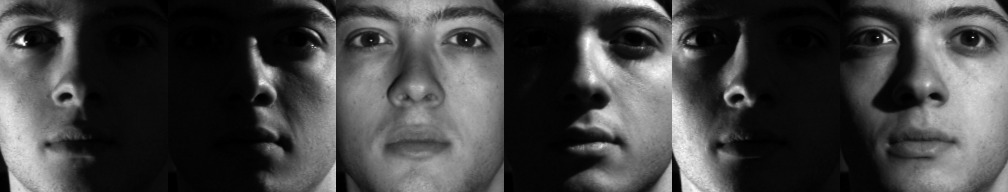
\includegraphics[width=\textwidth]{figures/person24trial1.jpg} 
\centering
\end{figure}

The analysis proceeded with running PCA on the images, then running RPCA with a variety of values for the $\lambda$ parameter (after some experimentation 0.001, 0.005, 0.01, and 0.02 were chosen as reasonably comprehensive values). After that, the original images were projected onto the eigenfaces produced from PCA and RPCA (going up to the eigenface that contained $90\%$ of the variance of the dataset in the PCA case. The graphs in the appendix demonstrate the silhouette of the resulting vectors, where the x axis the number of eigenfaces used in the projection, and the y axis is the silhouette score. Three difference distance metrics (cityblock, or $l1$-norm, euclidian, or $l2$-norm, and the cosine distance) were used. 

In general, RPCA performed slightly better than PCA, but not by a significant difference (it is barely noticable in the graphs). Neither PCA nor RPCA was capable of producing a silhouette score greater than zero, indicating that they did not map images of the same subject into appropriate clusters. The lambda value that performed best was $0.005$, and when lambda was $0.001$, the resulting low rank matrix lost enough of the features of the original images that the silhouette score plateaued after only around 11 eigenfaces.

As far as RRE scores, the relative error component was $4\%$ of the original dataset with $\lambda = 0.2$ and $59\%$ of the dataset when $\lambda = 0.001$.

\begin{figure}[H]
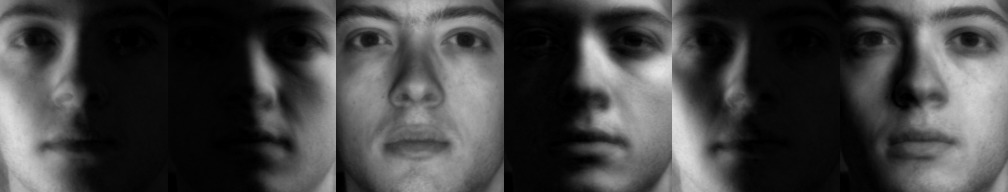
\includegraphics[width=\textwidth]{figures/person24Afterl=0dot005RPCAtrial1.jpg} 
\centering
\end{figure}

We can qualitatively analyze the images when the sparse error is removed from them to see what RPCA did accomplish, and why it did not result in the kind of improved eigenface performance we may have hoped. 

Here are the same faces shown above, but after the sparse error term has been removed by the IALM method (with $\lambda = 0.005$, or the best performing value of lambda). It's easy to see that the faces have had the specularities removed (in particular, note that the shine in the eyes has been removed). Clearly removing the sparse error inherent in these small abberations benefits us some, but it is not the dramatic change we would have hoped. Ideally, the shadows themselves could be considered error, and removed during the decomposition. Upon further consideration it seems that the shadows are themselves low rank, and thuis cannot be identified by the RPCA methodology as needing to be corrected. This explains why we didn't get the benefit we anticipated.

We can add a datapoint to our qualitative analysis somewhat by looking at what happened when we set $\lambda = 0.001$. In this case, the algorithm pays very little penality for making the 'sparse error' term relatively large (and in fact made a dramatic $59\%$ of the original images into the 'error'.

\begin{figure}[H]
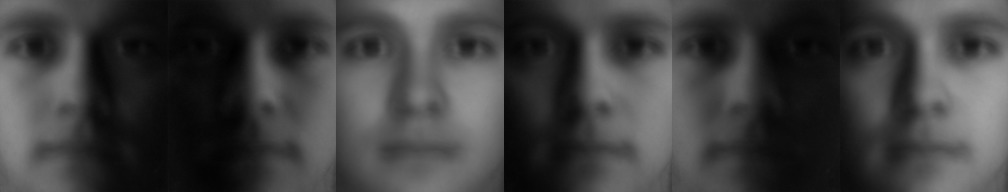
\includegraphics[width=\textwidth]{figures/person24Afterl=0dot001RPCAtrial1.jpg} 
\centering
\end{figure}

Here we can see that when given more leeway, the RPCA algorithm actually does an interesting thing, it begins to make the faces more similar to the eigenfaces, but keeps the various lighting conditions! This backs up our assertion that the reason that RPCA does not adequately improve performance when faced with various lightining conditions is that the lighting conditions are themselves low rank. If they were not, the RPCA algorithm would attempt to remove them.

Another interesting thing to note here (while not entirely relevant to RPCA) is that the euclidean distance metric was the best metric for the silhouette score here, but that none of the metrics were able to cross the 0 value. That is, no clustering was accomplished that adequately separated different indviduals using these methods.

\subsection{Trial 2: Bright dataset}

In an attempt to see whether RPCA added some value over PCA in slightly better conditions, the same analysis was rerun on a subset of the images that were not fully obscured or at very large angles. For the exact images one can look at the brightyalefaces/ directory in the github that supports this analysis, but here are five randomly selected images of the same subject from the second trial:

\begin{figure}[H]
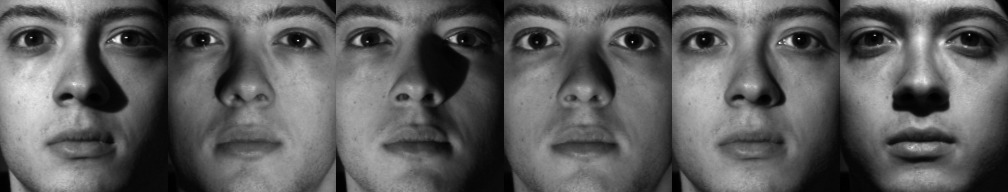
\includegraphics[width=\textwidth]{figures/person24trial2.jpg} 
\centering
\end{figure}

However, as can be seen in the appendix. this trial performed very similarly to the first, with the RPCA method offering little value over PCA. Interestingly in this case, the cosine metric performed most successfully in distinguishing images. While PCA did allow most of the variance (and the clustering) of the dataset to be translated into a \emph{much} smaller  number of dimension (~40 down from 32256, or $0.1\%$), RPCA did not add improve this reduction. It did however, yet again produce images that could qualitatively be said to have less small photographic aberrations. At the very least, RPCA serves as a reasonable selfie-filter.

\begin{figure}[H]
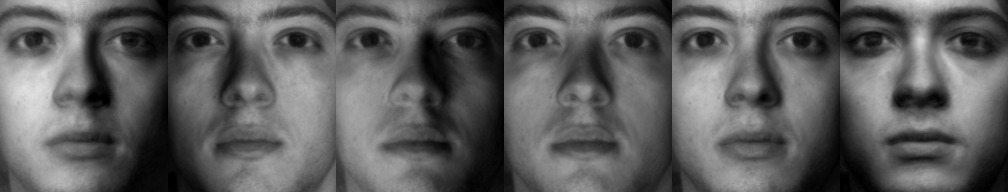
\includegraphics[width=\textwidth]{figures/person24Afterl=0dot005RPCAtrial2.jpg} 
\centering
\end{figure}

\subsection{Trial 3: Best dataset}

Finally, the same analysis was performed on only those images that were very well lit (which can be found in bestyalefaces/ in the attached github project). The results were very similar, but to quickly summarize: again cosine was the best separating metric, again RPCA performed negligibly better than PCA at producing eigenfaces that captured the data needed to distinguish individuals. 

\subsection{Video Segmentation Experiment Setup}

We used two different surveillance videos for experimenting background and foreground segmentation. The first video consists of a scene where a few birds move around in front of a largely white background. We cut a sequence of 36 frames from this video, each 1 second apart. The second video  displays a steady stream of cars moving down a highway. For traffic video, we cut a sequence of 31 frames from this video, each 1 second apart also. 

Background Truth for each video was constructed by manually removing all the sparse noise from a carefully selected frame. Due to slight variations of lighting and video quality across frames, this method did give us the exact Ground Truth. However, for the purpose of our analysis, this manually constructed Ground Truth was sufficient.

\subsection{Background and Foreground Modeling}
\bigskip
\begin{minipage}{\linewidth}
\bgroup
  \begin{tabular}{ | c | m{2.8cm} | m{2.8cm} | m{2.8cm} | }
    \hline
    Image Type & RPCA \linebreak (2PC, $\lambda$=0.015) & PCA \linebreak (1 PC) & PCA \linebreak (2 PC)
    \\ \hline
	Original \linebreak Image
    &
    \begin{minipage}{.3\textwidth}
      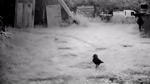
\includegraphics[width=\linewidth, width=25mm]{figures_video/crow/original.png}
    \end{minipage}
    & 
    \begin{minipage}{.3\textwidth}
      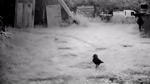
\includegraphics[width=\linewidth, width=25mm]{figures_video/crow/original.png}
    \end{minipage}
    &
    \begin{minipage}{.3\textwidth}
      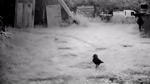
\includegraphics[width=\linewidth, width=25mm]{figures_video/crow/original.png}
    \end{minipage}
    \\ \hline
	Ground Truth (GT)
	&
    \begin{minipage}{.3\textwidth}
      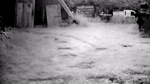
\includegraphics[width=\linewidth, width=25mm]{figures_video/crow/background.png}
    \end{minipage}
	&
    \begin{minipage}{.3\textwidth}
      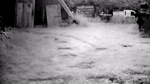
\includegraphics[width=\linewidth, width=25mm]{figures_video/crow/background.png}
    \end{minipage}
    &
    \begin{minipage}{.3\textwidth}
      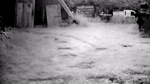
\includegraphics[width=\linewidth, width=25mm]{figures_video/crow/background.png}
    \end{minipage}
	\\ \hline
	
	Extracted Background (EB)
	&
    \begin{minipage}{.3\textwidth}
      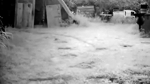
\includegraphics[width=\linewidth, width=25mm]{figures_video/crow/rpca/lowRank_0_015.png}
    \end{minipage}	
	&
    \begin{minipage}{.3\textwidth}
      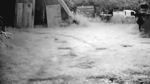
\includegraphics[width=\linewidth, width=25mm]{figures_video/crow/pca/lowRank_0.png}
    \end{minipage}
	&
    \begin{minipage}{.3\textwidth}
      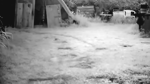
\includegraphics[width=\linewidth, width=25mm]{figures_video/crow/pca2/lowRank_0.png}
    \end{minipage}
	\\ \hline
	
	(GT - EB) Heatmap
	&
    \begin{minipage}{.3\textwidth}
      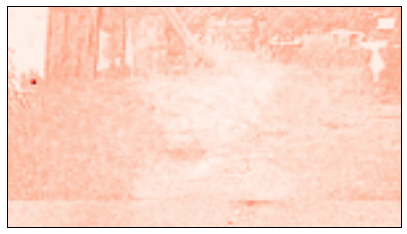
\includegraphics[width=\linewidth, width=25mm]{figures_video/crow/rpca/hm_0_015.png}
    \end{minipage}	
	&
    \begin{minipage}{.3\textwidth}
      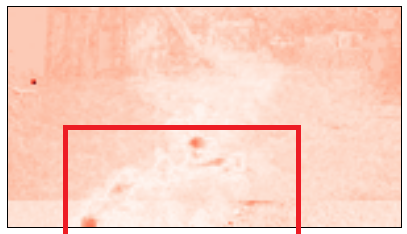
\includegraphics[width=\linewidth, width=25mm]{figures_video/crow/pca/hm_0.png}
    \end{minipage}		
	&
    \begin{minipage}{.3\textwidth}
      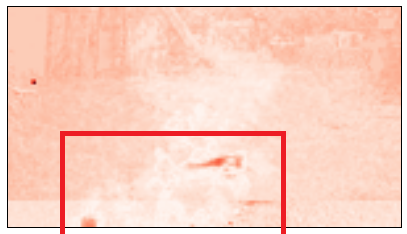
\includegraphics[width=\linewidth, width=25mm]{figures_video/crow/pca2/hm_0.png}
    \end{minipage}		
	\\ \hline	
	
	Foreground Noise
	&
    \begin{minipage}{.3\textwidth}
      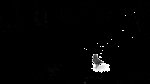
\includegraphics[width=\linewidth, width=25mm]{figures_video/crow/rpca/noise_0_015.png}
    \end{minipage}
	&
    \begin{minipage}{.3\textwidth}
      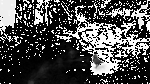
\includegraphics[width=\linewidth, width=25mm]{figures_video/crow/pca/noise_0.png}
    \end{minipage}
	&
    \begin{minipage}{.3\textwidth}
      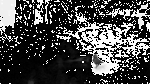
\includegraphics[width=\linewidth, width=25mm]{figures_video/crow/pca2/noise_0.png}
    \end{minipage}
	\\ \hline	
	
  \end{tabular}

\bigskip
\centerline{\textbf{Figure 6.6.1 Background and foreground segmentation on Bird Video }}
\centerline{\textbf{using RPCA and PCA}}
\bigskip
\egroup
\end{minipage}
As we can see from Figure 6.6.1 and Figure 6.6.2, the extracted background from RPCA for both bird and traffic videos more closely resembles background truth than that of PCA. There is a very minor trace of sparse noise in the extracted background and the differences are uniform throughout the image. Backgrounds extracted from PCA, however, suffers higher “pollution” caused by sparse noise present across the frames. The area with most visible difference is highlighted in red.

\bigskip
\begin{minipage}{\linewidth}
\bgroup
  \begin{tabular}{ | c | m{2.8cm} | m{2.8cm} | m{2.8cm} | }
    \hline
    Image Type & RPCA \linebreak (2PC, $\lambda$=0.007) & PCA \linebreak (1 PC) & PCA \linebreak (2 PC)
    \\ \hline
	Original \linebreak Image
    &
    \begin{minipage}{.3\textwidth}
      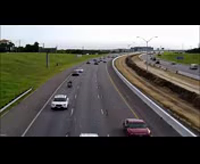
\includegraphics[width=\linewidth, width=25mm]{figures_video/traffic/original.png}
    \end{minipage}
    & 
    \begin{minipage}{.3\textwidth}
      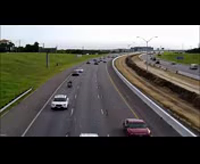
\includegraphics[width=\linewidth, width=25mm]{figures_video/traffic/original.png}
    \end{minipage}
    &
    \begin{minipage}{.3\textwidth}
      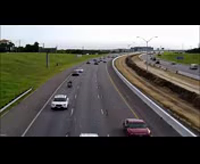
\includegraphics[width=\linewidth, width=25mm]{figures_video/traffic/original.png}
    \end{minipage}
    \\[5ex] \hline
	Ground Truth (GT)
	&
    \begin{minipage}{.3\textwidth}
      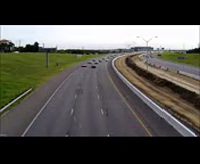
\includegraphics[width=\linewidth, width=25mm]{figures_video/traffic/background.png}
    \end{minipage}
	&
    \begin{minipage}{.3\textwidth}
      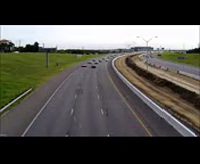
\includegraphics[width=\linewidth, width=25mm]{figures_video/traffic/background.png}
    \end{minipage}
    &
    \begin{minipage}{.3\textwidth}
      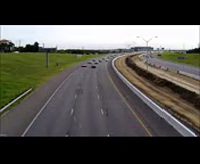
\includegraphics[width=\linewidth, width=25mm]{figures_video/traffic/background.png}
    \end{minipage}
	\\[5ex] \hline
	
	Extracted Background (EB)
	&
    \begin{minipage}{.3\textwidth}
      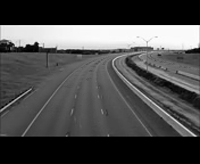
\includegraphics[width=\linewidth, width=25mm]{figures_video/traffic/rpca/lowRank_0.png}
    \end{minipage}	
	&
    \begin{minipage}{.3\textwidth}
      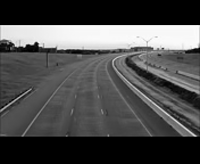
\includegraphics[width=\linewidth, width=25mm]{figures_video/traffic/pca/lowRank_0.png}
    \end{minipage}
	&
    \begin{minipage}{.3\textwidth}
      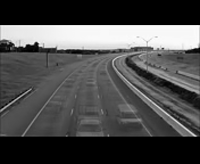
\includegraphics[width=\linewidth, width=25mm]{figures_video/traffic/pca2/lowRank_0.png}
    \end{minipage}
	\\[6ex] \hline
	
	(GT - EB) Heatmap
	&
    \begin{minipage}{.3\textwidth}
      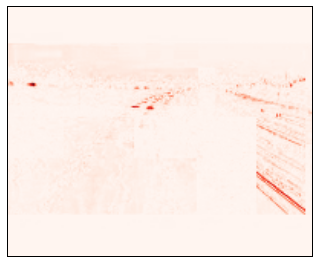
\includegraphics[width=\linewidth, width=25mm]{figures_video/traffic/rpca/hm_0.png}
    \end{minipage}	
	&
    \begin{minipage}{.3\textwidth}
      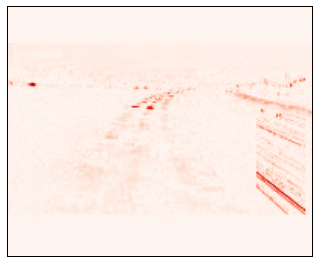
\includegraphics[width=\linewidth, width=25mm]{figures_video/traffic/pca/hm_0.png}
    \end{minipage}		
	&
    \begin{minipage}{.3\textwidth}
      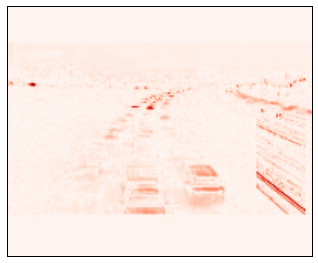
\includegraphics[width=\linewidth, width=25mm]{figures_video/traffic/pca2/hm_0.png}
    \end{minipage}		
	\\[6ex] \hline	
	
	Foreground Noise
	&
    \begin{minipage}{.3\textwidth}
      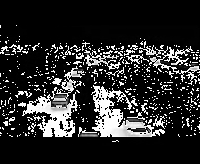
\includegraphics[width=\linewidth, width=25mm]{figures_video/traffic/rpca/noise_0.png}
    \end{minipage}
	&
    \begin{minipage}{.3\textwidth}
      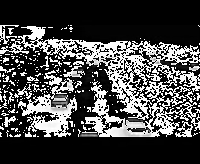
\includegraphics[width=\linewidth, width=25mm]{figures_video/traffic/pca/noise_0.png}
    \end{minipage}
	&
    \begin{minipage}{.3\textwidth}
      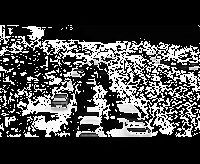
\includegraphics[width=\linewidth, width=25mm]{figures_video/traffic/pca2/noise_0.png}
    \end{minipage}
	\\[6ex] \hline	
	
  \end{tabular}

\bigskip
\centerline{\textbf{Figure 6.6.2 Background and foreground segmentation on Bird Video }}
\centerline{\textbf{using RPCA and PCA}}
\bigskip
\egroup
\end{minipage}
For foreground noise comparison, the Bird Video in Figure 6.6.1 provided a good visual on the difference between RPCA and PCA. RPCA managed to identify the exact pixel locations for foreground objects whereas PCA captured a mix of sparse noise and noise due to slight color variations in the frames. From here, we observed how RPCA prevented actual sparse noise from affecting our principal components without impacting the inherently Gaussian nature of the original data.

\centerline{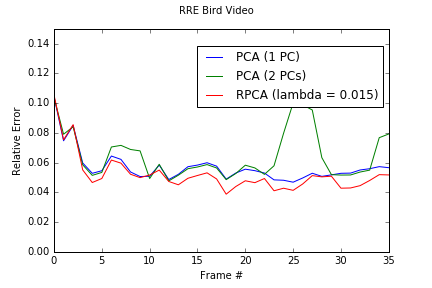
\includegraphics[width=\linewidth, width=100mm]{figures_video/crow/rre_015.png}}
\centerline{\textbf{Figure 6.6.3 Relative Reconstruction Error for Bird Video }}
\bigskip

Figure 6.6.3 shows the RRE for each background frame reconstructed from RPCA and PCA. Albeit a rough measure, we can see that RPCA’s extracted backgrounds are closer to Ground Truth than PCA, across almost all frames. Another interesting thing to note is that RRE for PCA using 2 components spiked for certain frames. The reason for this is that 2nd principal component was “used up” in explaining the variations cause by sparse noise, causing a big deviation of reconstructed background from the Ground Truth. The effect of sparse noise was exaggerated for this data but it highlighted the fact that for real life data using PCA for dimensionality reduction, certain noise/outlier can cause a major problem due to the inability of PCA to handle sparse noise.

\subsection{Impact of $\lambda$ on Background and Foreground Modeling}
Recall the equation for RPCA:
\[ \argmin_{M'}(||A||_* + \lambda||E||_1) \text{,  subject to  }  D = A + E \]

We were curious to know how $\lambda$ impacts the quality of our model and video segmentation provides a perfect opportunity to visualize this effect. Figure 6.6.4 shows the result for the Bird Video using $\lambda = 0.1$, instead of 0.015 as in Figure 6.6.1. With a large $\lambda$, RPCA’s performance in extracting background is roughly equivalent to naïve PCA. The impact of sparse noise on the extract background image for RPCA has also become apparent. The area of extracted foreground noise, on the other hand, is now much smaller and concentrated. With a large $\lambda$, RPCA is less aggressive in identifying noise and only large enough deviations from the Ground Truth are considered noise.
\bigskip

\begin{minipage}{\linewidth}
\bgroup
  \begin{tabular}{ | c | m{2.8cm} | m{2.8cm} | m{2.8cm} | }
    \hline
    Image Type & RPCA \linebreak (2PC, $\lambda$=0.06) & PCA \linebreak (1 PC) & PCA \linebreak (2 PC)
    \\ \hline
	Original \linebreak Image
    &
    \begin{minipage}{.3\textwidth}
      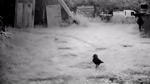
\includegraphics[width=\linewidth, width=25mm]{figures_video/crow/original.png}
    \end{minipage}
    & 
    \begin{minipage}{.3\textwidth}
      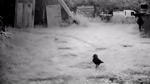
\includegraphics[width=\linewidth, width=25mm]{figures_video/crow/original.png}
    \end{minipage}
    &
    \begin{minipage}{.3\textwidth}
      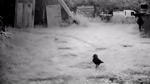
\includegraphics[width=\linewidth, width=25mm]{figures_video/crow/original.png}
    \end{minipage}
    \\ \hline
	Ground Truth (GT)
	&
    \begin{minipage}{.3\textwidth}
      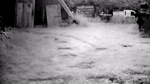
\includegraphics[width=\linewidth, width=25mm]{figures_video/crow/background.png}
    \end{minipage}
	&
    \begin{minipage}{.3\textwidth}
      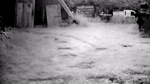
\includegraphics[width=\linewidth, width=25mm]{figures_video/crow/background.png}
    \end{minipage}
    &
    \begin{minipage}{.3\textwidth}
      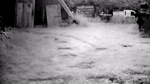
\includegraphics[width=\linewidth, width=25mm]{figures_video/crow/background.png}
    \end{minipage}
	\\ \hline
	
	Extracted Background (EB)
	&
    \begin{minipage}{.3\textwidth}
      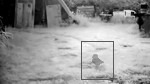
\includegraphics[width=\linewidth, width=25mm]{figures_video/crow/rpca/lowRank_0_06.png}
    \end{minipage}	
	&
    \begin{minipage}{.3\textwidth}
      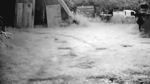
\includegraphics[width=\linewidth, width=25mm]{figures_video/crow/pca/lowRank_0.png}
    \end{minipage}
	&
    \begin{minipage}{.3\textwidth}
      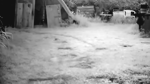
\includegraphics[width=\linewidth, width=25mm]{figures_video/crow/pca2/lowRank_0.png}
    \end{minipage}
	\\ \hline
	
	(GT - EB) Heatmap
	&
    \begin{minipage}{.3\textwidth}
      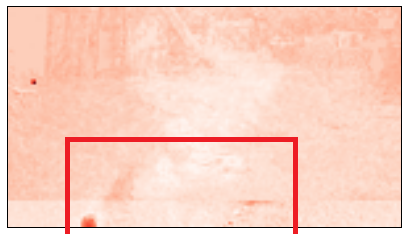
\includegraphics[width=\linewidth, width=25mm]{figures_video/crow/rpca/hm_0_06.png}
    \end{minipage}	
	&
    \begin{minipage}{.3\textwidth}
      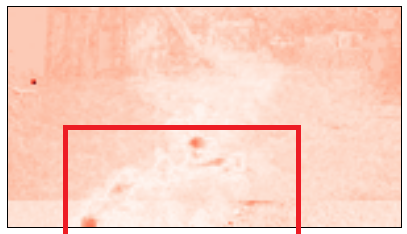
\includegraphics[width=\linewidth, width=25mm]{figures_video/crow/pca/hm_0.png}
    \end{minipage}		
	&
    \begin{minipage}{.3\textwidth}
      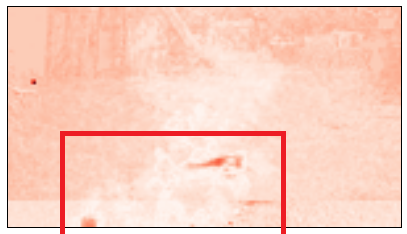
\includegraphics[width=\linewidth, width=25mm]{figures_video/crow/pca2/hm_0.png}
    \end{minipage}		
	\\ \hline	
	
	Foreground Noise
	&
    \begin{minipage}{.3\textwidth}
      
\includegraphics[width=\linewidth, width=25mm]{figures_video/crow/rpca/noise_0_06.png}
    \end{minipage}
	&
    \begin{minipage}{.3\textwidth}
      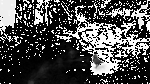
\includegraphics[width=\linewidth, width=25mm]{figures_video/crow/pca/noise_0.png}
    \end{minipage}
	&
    \begin{minipage}{.3\textwidth}
      \includegraphics[width=\linewidth, width=25mm]{figures_video/crow/pca2/noise_0.png}
    \end{minipage}
	\\ \hline	
	
  \end{tabular}

\bigskip
\centerline{\textbf{Figure 6.6.4 Segmentation on Bird Video wtih $\lambda = 0.06$ }}
\egroup
\end{minipage}
\centerline{\includegraphics[width=\linewidth, width=100mm]{figures_video/crow/rre_006.png}}
\centerline{\textbf{Figure 6.6.3 Relative Reconstruction Error for Bird Video with $\lambda=0.06$ }}
\bigskip

\section{Conclusion}

We have analyzed the use of RPCA in two separate domains: for facial recognition and for video segmentation. Our results show that while it has been said to have uses in the former domain, the fact that facial shadowing is itself low rank, it does not effectively separate that out, and in fact performs only marginally better than PCA (and certainly not enough to justify the longer processing time). However, in the latter case of video segementation, it performed quitre well.

Based on the above experiments, we observed that RPCA is useful for removing irregularities in our dataset and therefore can help PCA obtain a good model governing the data. However, what makes RPCA effective is the regularization parameter lambda that controls how much noise to be removed. In addition, it is important that RPCA be applied in circumstances where the error is of a type that the method will recognize. Like any other machine learning technique, the first step towards effective dimensionality reduction is to understand the nature of our dataset and apply RPCA appropriately.

\newpage

\section{Appendix}

\subsection{Trial 1 - Graphs}

\begin{figure}[H]
\centering
\includegraphics[width=0.6\textwidth]{figures/rpcatrial1cityblock.png}\\
\includegraphics[width=0.6\textwidth]{figures/rpcatrial1cosine.png}\\
\includegraphics[width=0.6\textwidth]{figures/rpcatrial1euclidean.png}\\
\end{figure}

\subsection{Trial 2- Graphs}

\begin{figure}[H]
\centering
\includegraphics[width=0.6\textwidth]{figures/rpcatrial2cityblock.png}\\
\includegraphics[width=0.6\textwidth]{figures/rpcatrial2cosine.png}\\
\includegraphics[width=0.6\textwidth]{figures/rpcatrial2euclidean.png}\\
\end{figure}

\subsection{Trial3- Graphs}

\begin{figure}[H]
\centering
\includegraphics[width=0.6\textwidth]{figures/rpcatrial3cityblock.png}\\
\includegraphics[width=0.6\textwidth]{figures/rpcatrial3cosine.png}\\
\includegraphics[width=0.6\textwidth]{figures/rpcatrial3euclidean.png}\\
\end{figure}


\begin{thebibliography}{9}

\bibitem{lambertian} Basri, R., \& Jacobs, D. W. (2003). Lambertian reflectance and linear subspaces. IEEE transactions on pattern analysis and machine intelligence, 25(2), 218-233.

\bibitem{pcp} Candès, E. J., Li, X., Ma, Y., \& Wright, J. (2011). Robust principal component analysis?. Journal of the ACM (JACM), 58(3), 11.

\bibitem{incoherence} Candes, E., \& Recht, B. (2012). Exact matrix completion via convex optimization. Communications of the ACM, 55(6), 111-119.

\bibitem{pca} Eckart, C., \& Young, G. (1936). The approximation of one matrix by another of lower rank. Psychometrika, 1(3), 211-218.

\bibitem{yaleb} Georghiades, A. S., Belhumeur, P. N., \& Kriegman, D. J. (2001). From few to many: Illumination cone models for face recognition under variable lighting and pose. IEEE transactions on pattern analysis and machine intelligence, 23(6), 643-660.

\bibitem{usedcode} Kastner, K. (2014) "Robust Matrix Decomposition." Garbage In Garbage Out. http://kastnerkyle.github.io/posts/robust-matrix-decomposition/

\bibitem{croppedyaleb} Lee, K. C., Ho, J., \& Kriegman, D. J. (2005). Acquiring linear subspaces for face recognition under variable lighting. IEEE Transactions on pattern analysis and machine intelligence, 27(5), 684-698.

\bibitem{iaml} Lin, Z., Chen, M., \& Ma, Y. (2010). The augmented lagrange multiplier method for exact recovery of corrupted low-rank matrices. arXiv preprint arXiv:1009.5055.

\bibitem{scikit} Pedregosa, F., Varoquaux, G., Gramfort, A., Michel, V., Thirion, B., Grisel, O., ... \& Vanderplas, J. (2011). Scikit-learn: Machine learning in Python. Journal of Machine Learning Research, 12(Oct), 2825-2830.

\bibitem{silhouette} Rousseeuw, P. J. (1987). Silhouettes: a graphical aid to the interpretation and validation of cluster analysis. Journal of computational and applied mathematics, 20, 53-65.

\bibitem{rpca} Wright, J., Ganesh, A., Rao, S., Peng, Y., \& Ma, Y. (2009). Robust principal component analysis: Exact recovery of corrupted low-rank matrices via convex optimization. In Advances in neural information processing systems (pp. 2080-2088).

\end{thebibliography}
\end{document}

